\documentclass[crop,class=article]{standalone}
%----------------------------Preamble-------------------------------%
\usepackage{tikz}                       % Drawing/graphing tools.
\usetikzlibrary{
    arrows.meta,            % For Latex Arrows.
    decorations.markings    % Adding arrows in the middle of a line.
}
%--------------------------Main Document----------------------------%
\begin{document}
    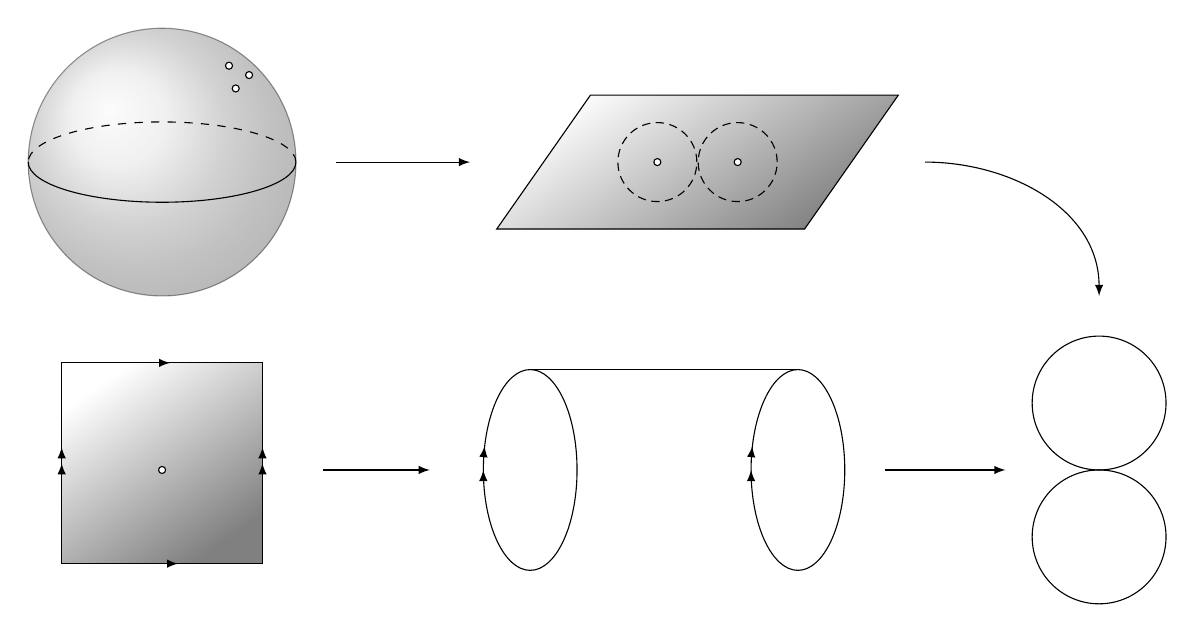
\begin{tikzpicture}[%
        every edge/.style={draw=black},
        scale=1.7,
        >=latex
    ]
        \draw[ball color=gray!40, opacity=0.4] (0,0) circle (1cm);
        \draw (-1,0) arc (180:360:1 and 0.3);
        \draw[dashed] (1,0) arc (0:180:1 and 0.3);
        \draw[fill=white] (0.55,0.55) circle (0.75pt);
        \draw[fill=white] (0.65,0.65) circle (0.75pt);
        \draw[fill=white] (0.5,0.72)  circle (0.75pt);
        \draw[->] (1.3,0) to (2.3,0);
        \draw[fill=gray, shading angle=215]
            (2.5,-0.5)--(3.2,0.5)--(5.5,0.5)--(4.8,-0.5)--cycle;
        \draw[densely dashed] (3.7,0) circle (0.295);
        \draw[densely dashed] (4.3,0) circle (0.295);
        \draw[fill=white] (3.7,0) circle (0.75pt);
        \draw[fill=white] (4.3,0) circle (0.75pt);
        \draw[->] (5.7,0) to [in=90,out=0] (7,-1);
        \draw[->] (1.2,-2.3)--(2,-2.3);
        \draw[%
            postaction={decorate},
            decoration={%
                markings,
                mark=at position .145 with \arrow{latex},
                mark=at position .375 with \arrow{latex},
                mark=at position .395 with \arrow{latex},
                mark=at position .615 with \arrowreversed{latex},
                mark=at position .855 with \arrowreversed{latex},
                mark=at position .875 with \arrowreversed{latex}
            },
            fill=gray,
            shading angle=215
        ] (-0.75,-3)--(0.75,-3)--(0.75,-1.5)--(-0.75,-1.5)--cycle;
        \draw[fill=white] (0,-2.3) circle (0.75pt);
        \draw[%
            postaction={decorate},
            decoration={%
                markings,
                mark=at position .5 with \arrow{latex},
                mark=at position .55 with \arrow{latex}
            }
        ]   (3.1,-2.3) arc[%
                    start angle=0,
                    delta angle=-360,
                    x radius=.35,
                    y radius=.75
            ];
        \draw (2.75,-1.55) -- (4.75,-1.55);
        \draw[%
            postaction={decorate},
            decoration={%
            markings,
            mark=at position .5 with \arrow{latex},
            mark=at position .55 with \arrow{latex}
            }
        ]   (5.1cm,-2.3cm) arc[%
                start angle=0,
                delta angle=-360,
                x radius=.35,
                y radius=.75
            ];
        \draw[->] (5.4,-2.3)--(6.3,-2.3);
        \draw (7,-1.8) circle (0.5);
        \draw (7,-2.8) circle (0.5);
    \end{tikzpicture}
\end{document}